% Auto-generated from docs/schematic/spec_protocol.py via render.py — edit the template, not the .tex.
\documentclass[tikz,border=6pt]{standalone}
\usepackage{amsmath}
\usepackage{tikz}
\usetikzlibrary{arrows.meta,calc}
\definecolor{plasticcol}{HTML}{4C8DFF}
\definecolor{frozencol}{HTML}{9AA0A6}
\definecolor{predcol}{HTML}{4C8DFF}
\definecolor{errcol}{HTML}{E0772B}
\definecolor{nodestroke}{HTML}{222222}
\definecolor{shadecol}{HTML}{3C4043}
\definecolor{clampcol}{HTML}{222222}
\definecolor{titlecol}{HTML}{222222}
\definecolor{mutedcol}{HTML}{6B7075}
% a small padlock at coordinate #1 in colour #2 — marks frozen weights
\newcommand{\padlock}[2]{%
  \begin{scope}[shift={#1}, draw=#2, line width=0.8pt, line join=round]
    \draw (-0.06,0.05) -- (-0.06,0.11) arc (180:0:0.06) -- (0.06,0.05); % shackle
    \fill[#2] (-0.11,-0.13) rectangle (0.11,0.05);                      % body
    \fill[white] (0,-0.03) circle (0.023);                             % keyhole
  \end{scope}}
\begin{document}
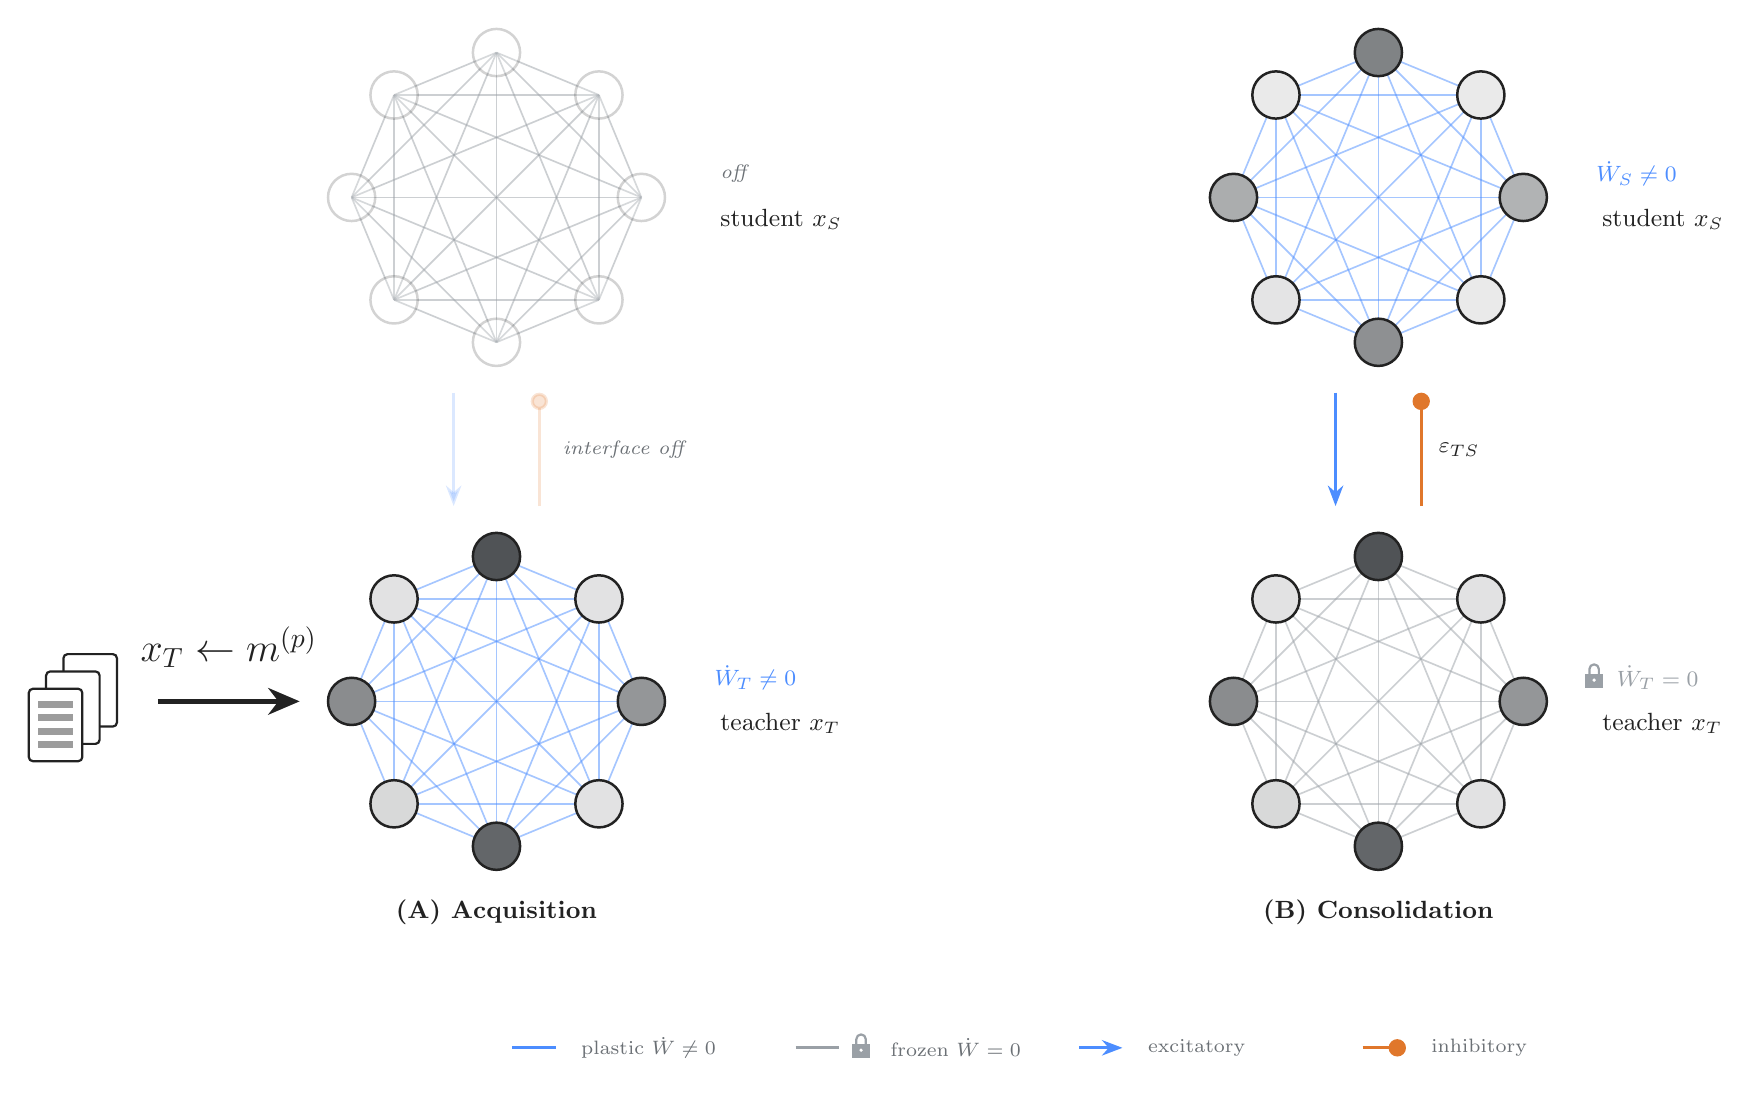
\begin{tikzpicture}[
  node/.style={circle, draw=nodestroke, line width=0.9pt, minimum size=6mm, inner sep=0pt},
  mesh/.style={line width=0.6pt, opacity=0.5},
  chord/.style={line width=1.15pt},
  excit/.style={-{Stealth[length=2.6mm]}},
  inhib/.style={-{Circle[length=2.2mm, width=2.2mm]}},
  poplab/.style={font=\small, text=titlecol},
  wlab/.style={font=\footnotesize, text=titlecol, fill=white, inner sep=1.2pt},
  offlab/.style={font=\scriptsize\itshape, text=mutedcol},
  title/.style={font=\small\bfseries, text=titlecol},
  clab/.style={font=\footnotesize, text=clampcol, fill=white, inner sep=1.2pt},
  lgd/.style={font=\scriptsize, text=mutedcol},
]


% =================== PANEL A : Acquisition ===================

% ---- teacher ring (state: plastic) ----


% recurrent weights W_T: complete graph, drawn as a mesh BEHIND the nodes

\draw[mesh, plasticcol] (0.000,-4.560) -- (1.301,-5.099);

\draw[mesh, plasticcol] (0.000,-4.560) -- (1.840,-6.400);

\draw[mesh, plasticcol] (0.000,-4.560) -- (1.301,-7.701);

\draw[mesh, plasticcol] (0.000,-4.560) -- (0.000,-8.240);

\draw[mesh, plasticcol] (0.000,-4.560) -- (-1.301,-7.701);

\draw[mesh, plasticcol] (0.000,-4.560) -- (-1.840,-6.400);

\draw[mesh, plasticcol] (0.000,-4.560) -- (-1.301,-5.099);

\draw[mesh, plasticcol] (1.301,-5.099) -- (1.840,-6.400);

\draw[mesh, plasticcol] (1.301,-5.099) -- (1.301,-7.701);

\draw[mesh, plasticcol] (1.301,-5.099) -- (0.000,-8.240);

\draw[mesh, plasticcol] (1.301,-5.099) -- (-1.301,-7.701);

\draw[mesh, plasticcol] (1.301,-5.099) -- (-1.840,-6.400);

\draw[mesh, plasticcol] (1.301,-5.099) -- (-1.301,-5.099);

\draw[mesh, plasticcol] (1.840,-6.400) -- (1.301,-7.701);

\draw[mesh, plasticcol] (1.840,-6.400) -- (0.000,-8.240);

\draw[mesh, plasticcol] (1.840,-6.400) -- (-1.301,-7.701);

\draw[mesh, plasticcol] (1.840,-6.400) -- (-1.840,-6.400);

\draw[mesh, plasticcol] (1.840,-6.400) -- (-1.301,-5.099);

\draw[mesh, plasticcol] (1.301,-7.701) -- (0.000,-8.240);

\draw[mesh, plasticcol] (1.301,-7.701) -- (-1.301,-7.701);

\draw[mesh, plasticcol] (1.301,-7.701) -- (-1.840,-6.400);

\draw[mesh, plasticcol] (1.301,-7.701) -- (-1.301,-5.099);

\draw[mesh, plasticcol] (0.000,-8.240) -- (-1.301,-7.701);

\draw[mesh, plasticcol] (0.000,-8.240) -- (-1.840,-6.400);

\draw[mesh, plasticcol] (0.000,-8.240) -- (-1.301,-5.099);

\draw[mesh, plasticcol] (-1.301,-7.701) -- (-1.840,-6.400);

\draw[mesh, plasticcol] (-1.301,-7.701) -- (-1.301,-5.099);

\draw[mesh, plasticcol] (-1.840,-6.400) -- (-1.301,-5.099);


\node[node, fill=shadecol!90] (A-T0) at (0.000,-4.560) {};

\node[node, fill=shadecol!15] (A-T1) at (1.301,-5.099) {};

\node[node, fill=shadecol!55] (A-T2) at (1.840,-6.400) {};

\node[node, fill=shadecol!15] (A-T3) at (1.301,-7.701) {};

\node[node, fill=shadecol!80] (A-T4) at (0.000,-8.240) {};

\node[node, fill=shadecol!20] (A-T5) at (-1.301,-7.701) {};

\node[node, fill=shadecol!60] (A-T6) at (-1.840,-6.400) {};

\node[node, fill=shadecol!15] (A-T7) at (-1.301,-5.099) {};


% teacher recurrent-weight tag


\node[wlab, text=plasticcol, anchor=west] at (2.720,-6.100) {$\dot W_T\neq0$};

\node[poplab, anchor=west] at (2.720,-6.680) {teacher $x_T$};

% ---- student ring (state: off) ----

\begin{scope}[opacity=0.2]
% recurrent weights W_S: complete graph, drawn as a mesh BEHIND the nodes

\draw[mesh, frozencol] (0.000,1.840) -- (1.301,1.301);

\draw[mesh, frozencol] (0.000,1.840) -- (1.840,-0.000);

\draw[mesh, frozencol] (0.000,1.840) -- (1.301,-1.301);

\draw[mesh, frozencol] (0.000,1.840) -- (0.000,-1.840);

\draw[mesh, frozencol] (0.000,1.840) -- (-1.301,-1.301);

\draw[mesh, frozencol] (0.000,1.840) -- (-1.840,-0.000);

\draw[mesh, frozencol] (0.000,1.840) -- (-1.301,1.301);

\draw[mesh, frozencol] (1.301,1.301) -- (1.840,-0.000);

\draw[mesh, frozencol] (1.301,1.301) -- (1.301,-1.301);

\draw[mesh, frozencol] (1.301,1.301) -- (0.000,-1.840);

\draw[mesh, frozencol] (1.301,1.301) -- (-1.301,-1.301);

\draw[mesh, frozencol] (1.301,1.301) -- (-1.840,-0.000);

\draw[mesh, frozencol] (1.301,1.301) -- (-1.301,1.301);

\draw[mesh, frozencol] (1.840,-0.000) -- (1.301,-1.301);

\draw[mesh, frozencol] (1.840,-0.000) -- (0.000,-1.840);

\draw[mesh, frozencol] (1.840,-0.000) -- (-1.301,-1.301);

\draw[mesh, frozencol] (1.840,-0.000) -- (-1.840,-0.000);

\draw[mesh, frozencol] (1.840,-0.000) -- (-1.301,1.301);

\draw[mesh, frozencol] (1.301,-1.301) -- (0.000,-1.840);

\draw[mesh, frozencol] (1.301,-1.301) -- (-1.301,-1.301);

\draw[mesh, frozencol] (1.301,-1.301) -- (-1.840,-0.000);

\draw[mesh, frozencol] (1.301,-1.301) -- (-1.301,1.301);

\draw[mesh, frozencol] (0.000,-1.840) -- (-1.301,-1.301);

\draw[mesh, frozencol] (0.000,-1.840) -- (-1.840,-0.000);

\draw[mesh, frozencol] (0.000,-1.840) -- (-1.301,1.301);

\draw[mesh, frozencol] (-1.301,-1.301) -- (-1.840,-0.000);

\draw[mesh, frozencol] (-1.301,-1.301) -- (-1.301,1.301);

\draw[mesh, frozencol] (-1.840,-0.000) -- (-1.301,1.301);


\node[node, fill=shadecol!0] (A-S0) at (0.000,1.840) {};

\node[node, fill=shadecol!0] (A-S1) at (1.301,1.301) {};

\node[node, fill=shadecol!0] (A-S2) at (1.840,-0.000) {};

\node[node, fill=shadecol!0] (A-S3) at (1.301,-1.301) {};

\node[node, fill=shadecol!0] (A-S4) at (0.000,-1.840) {};

\node[node, fill=shadecol!0] (A-S5) at (-1.301,-1.301) {};

\node[node, fill=shadecol!0] (A-S6) at (-1.840,-0.000) {};

\node[node, fill=shadecol!0] (A-S7) at (-1.301,1.301) {};

\end{scope}
% student recurrent-weight tag


\node[offlab, anchor=west] at (2.720,0.300) {off};

\node[poplab, anchor=west] at (2.720,-0.280) {student $x_S$};

% ---- teacher <-> student interface (state: off) ----


\begin{scope}[opacity=0.2]
\draw[predcol, chord, excit] (-0.544,-2.480) -- (-0.544,-3.920);
\draw[errcol, chord, inhib] (0.544,-3.920) -- (0.544,-2.480);
\end{scope}
\node[offlab, anchor=west] at (0.720,-3.200) {interface off};


% ---- clamp x_T <- m^(p): a roomy stack of interleaved memory patterns + a bold arrow ----


% interleaved stack, back-to-front (offset up-right); front card carries a pattern hint
\foreach \d in {0.44,0.22,0}{
  \draw[clampcol, line width=0.8pt, fill=white, rounded corners=1.5pt]
     (-5.60+\d-0.34,-6.700+\d-0.46) rectangle (-5.60+\d+0.34,-6.700+\d+0.46);}
\foreach \k in {0.26,0.09,-0.08,-0.25}{
  \fill[clampcol!45] (-5.60-0.22,-6.700+\k-0.045) rectangle (-5.60+0.22,-6.700+\k+0.045);}
% bold clamp arrow into the teacher-left node
\draw[clampcol, line width=1.6pt, -{Stealth[length=4mm,width=3.4mm]}]
   (-4.3,-6.400) -- (-2.5,-6.400);
\node[font=\Large, text=clampcol, anchor=south] at (-3.4,-6.1) {$x_T\leftarrow m^{(p)}$};


% ---- panel title ----
\node[title, anchor=north] at (0.000,-8.800) {(A) Acquisition};

% =================== PANEL B : Consolidation ===================

% ---- teacher ring (state: frozen) ----


% recurrent weights W_T: complete graph, drawn as a mesh BEHIND the nodes

\draw[mesh, frozencol] (11.200,-4.560) -- (12.501,-5.099);

\draw[mesh, frozencol] (11.200,-4.560) -- (13.040,-6.400);

\draw[mesh, frozencol] (11.200,-4.560) -- (12.501,-7.701);

\draw[mesh, frozencol] (11.200,-4.560) -- (11.200,-8.240);

\draw[mesh, frozencol] (11.200,-4.560) -- (9.899,-7.701);

\draw[mesh, frozencol] (11.200,-4.560) -- (9.360,-6.400);

\draw[mesh, frozencol] (11.200,-4.560) -- (9.899,-5.099);

\draw[mesh, frozencol] (12.501,-5.099) -- (13.040,-6.400);

\draw[mesh, frozencol] (12.501,-5.099) -- (12.501,-7.701);

\draw[mesh, frozencol] (12.501,-5.099) -- (11.200,-8.240);

\draw[mesh, frozencol] (12.501,-5.099) -- (9.899,-7.701);

\draw[mesh, frozencol] (12.501,-5.099) -- (9.360,-6.400);

\draw[mesh, frozencol] (12.501,-5.099) -- (9.899,-5.099);

\draw[mesh, frozencol] (13.040,-6.400) -- (12.501,-7.701);

\draw[mesh, frozencol] (13.040,-6.400) -- (11.200,-8.240);

\draw[mesh, frozencol] (13.040,-6.400) -- (9.899,-7.701);

\draw[mesh, frozencol] (13.040,-6.400) -- (9.360,-6.400);

\draw[mesh, frozencol] (13.040,-6.400) -- (9.899,-5.099);

\draw[mesh, frozencol] (12.501,-7.701) -- (11.200,-8.240);

\draw[mesh, frozencol] (12.501,-7.701) -- (9.899,-7.701);

\draw[mesh, frozencol] (12.501,-7.701) -- (9.360,-6.400);

\draw[mesh, frozencol] (12.501,-7.701) -- (9.899,-5.099);

\draw[mesh, frozencol] (11.200,-8.240) -- (9.899,-7.701);

\draw[mesh, frozencol] (11.200,-8.240) -- (9.360,-6.400);

\draw[mesh, frozencol] (11.200,-8.240) -- (9.899,-5.099);

\draw[mesh, frozencol] (9.899,-7.701) -- (9.360,-6.400);

\draw[mesh, frozencol] (9.899,-7.701) -- (9.899,-5.099);

\draw[mesh, frozencol] (9.360,-6.400) -- (9.899,-5.099);


\node[node, fill=shadecol!90] (B-T0) at (11.200,-4.560) {};

\node[node, fill=shadecol!15] (B-T1) at (12.501,-5.099) {};

\node[node, fill=shadecol!55] (B-T2) at (13.040,-6.400) {};

\node[node, fill=shadecol!15] (B-T3) at (12.501,-7.701) {};

\node[node, fill=shadecol!80] (B-T4) at (11.200,-8.240) {};

\node[node, fill=shadecol!20] (B-T5) at (9.899,-7.701) {};

\node[node, fill=shadecol!60] (B-T6) at (9.360,-6.400) {};

\node[node, fill=shadecol!15] (B-T7) at (9.899,-5.099) {};


% teacher recurrent-weight tag


\padlock{ (13.940,-6.100) }{frozencol}
\node[wlab, text=frozencol, anchor=west] at (14.180,-6.100) {$\dot W_T=0$};

\node[poplab, anchor=west] at (13.920,-6.680) {teacher $x_T$};

% ---- student ring (state: plastic) ----


% recurrent weights W_S: complete graph, drawn as a mesh BEHIND the nodes

\draw[mesh, plasticcol] (11.200,1.840) -- (12.501,1.301);

\draw[mesh, plasticcol] (11.200,1.840) -- (13.040,-0.000);

\draw[mesh, plasticcol] (11.200,1.840) -- (12.501,-1.301);

\draw[mesh, plasticcol] (11.200,1.840) -- (11.200,-1.840);

\draw[mesh, plasticcol] (11.200,1.840) -- (9.899,-1.301);

\draw[mesh, plasticcol] (11.200,1.840) -- (9.360,-0.000);

\draw[mesh, plasticcol] (11.200,1.840) -- (9.899,1.301);

\draw[mesh, plasticcol] (12.501,1.301) -- (13.040,-0.000);

\draw[mesh, plasticcol] (12.501,1.301) -- (12.501,-1.301);

\draw[mesh, plasticcol] (12.501,1.301) -- (11.200,-1.840);

\draw[mesh, plasticcol] (12.501,1.301) -- (9.899,-1.301);

\draw[mesh, plasticcol] (12.501,1.301) -- (9.360,-0.000);

\draw[mesh, plasticcol] (12.501,1.301) -- (9.899,1.301);

\draw[mesh, plasticcol] (13.040,-0.000) -- (12.501,-1.301);

\draw[mesh, plasticcol] (13.040,-0.000) -- (11.200,-1.840);

\draw[mesh, plasticcol] (13.040,-0.000) -- (9.899,-1.301);

\draw[mesh, plasticcol] (13.040,-0.000) -- (9.360,-0.000);

\draw[mesh, plasticcol] (13.040,-0.000) -- (9.899,1.301);

\draw[mesh, plasticcol] (12.501,-1.301) -- (11.200,-1.840);

\draw[mesh, plasticcol] (12.501,-1.301) -- (9.899,-1.301);

\draw[mesh, plasticcol] (12.501,-1.301) -- (9.360,-0.000);

\draw[mesh, plasticcol] (12.501,-1.301) -- (9.899,1.301);

\draw[mesh, plasticcol] (11.200,-1.840) -- (9.899,-1.301);

\draw[mesh, plasticcol] (11.200,-1.840) -- (9.360,-0.000);

\draw[mesh, plasticcol] (11.200,-1.840) -- (9.899,1.301);

\draw[mesh, plasticcol] (9.899,-1.301) -- (9.360,-0.000);

\draw[mesh, plasticcol] (9.899,-1.301) -- (9.899,1.301);

\draw[mesh, plasticcol] (9.360,-0.000) -- (9.899,1.301);


\node[node, fill=shadecol!65] (B-S0) at (11.200,1.840) {};

\node[node, fill=shadecol!11] (B-S1) at (12.501,1.301) {};

\node[node, fill=shadecol!40] (B-S2) at (13.040,-0.000) {};

\node[node, fill=shadecol!11] (B-S3) at (12.501,-1.301) {};

\node[node, fill=shadecol!58] (B-S4) at (11.200,-1.840) {};

\node[node, fill=shadecol!14] (B-S5) at (9.899,-1.301) {};

\node[node, fill=shadecol!43] (B-S6) at (9.360,-0.000) {};

\node[node, fill=shadecol!11] (B-S7) at (9.899,1.301) {};


% student recurrent-weight tag


\node[wlab, text=plasticcol, anchor=west] at (13.920,0.300) {$\dot W_S\neq0$};

\node[poplab, anchor=west] at (13.920,-0.280) {student $x_S$};

% ---- teacher <-> student interface (state: on) ----



\draw[predcol, chord, excit] (10.656,-2.480) -- (10.656,-3.920);
\draw[errcol, chord, inhib] (11.744,-3.920) -- (11.744,-2.480);

\node[wlab, anchor=west] at (11.920,-3.200) {$\varepsilon_{TS}$};


% ---- clamp x_T <- m^(p): a roomy stack of interleaved memory patterns + a bold arrow ----


% ---- panel title ----
\node[title, anchor=north] at (11.200,-8.800) {(B) Consolidation};


% =================== legend (centred under the two panels, generous pitch) ===================


\draw[plasticcol, chord] (0.200,-10.800) -- ++(0.55,0);
\node[lgd, anchor=west] at (0.950,-10.800) {plastic $\dot W\neq0$};
\draw[frozencol, chord] (3.800,-10.800) -- ++(0.55,0);
\padlock{ (4.630,-10.800) }{frozencol}
\node[lgd, anchor=west] at (4.880,-10.800) {frozen $\dot W=0$};
\draw[predcol, chord, excit] (7.400,-10.800) -- ++(0.55,0);
\node[lgd, anchor=west] at (8.150,-10.800) {excitatory};
\draw[errcol, chord, inhib] (11.000,-10.800) -- ++(0.55,0);
\node[lgd, anchor=west] at (11.750,-10.800) {inhibitory};
\end{tikzpicture}
\end{document}